%%%%%%%%%%%%%%%%%%%%%%%%%%%%%
%% Styles, packages and new commands
\input{../../Main/ML_Main.tex}
%%%%%%%%%%%%%%%%%%%%%%%%%%%%%
%% Edit the title page
\title{Machine Learning}
\subtitle{Module 8.2 - Unsupervised Learning: Dimension Reduction}
\author[MOB]{Marc-Olivier Boldi}
\institute[HEC MSc Mgt BA]{Master in Management, Business Analytics, HEC UNIL}
\date{Spring 2025}
%%%%%%%%%%%%%%%%%%%%%%%%%%%%%
%%%%%%%%%%%%%%%%%%%%%%%%%%%%%
%%%%%%%%%%%%%%%%%%%%%%%%%%%%%
%%%%%%%%%%%%%%%%%%%%%%%%%%%%%
\begin{document}
%%%%%%%%%%%%%%%%%%%%%%%%%%%%%
\begin{frame}
  \titlepage
\end{frame}
%%%%%%%%%%%%%%%%%%%%%%%%%%%%%
\begin{frame}
\frametitle{Table of Contents}
	\tableofcontents
\end{frame}
%%%%%%%%%%%%%%%%%%%%%%%%%%%%%
\section{Dimension reduction}
%%%%%%%%%%%%%%%%%%%%%%%%%%%%%
\begin{frame}
\frametitle{Concept}
For unsupervised learning, {\bf data representation and simplification} is an important task. A natural objective is to represent the data on a graph: simplify $p$ features to 2 dimensions and plot on $x$- and $y$-axes. \\
\vspace{0.2cm}
{\bf Example:} {\tt iris} data has $4$ features (species not used). The data cannot be represented on a single graph.
\begin{center}
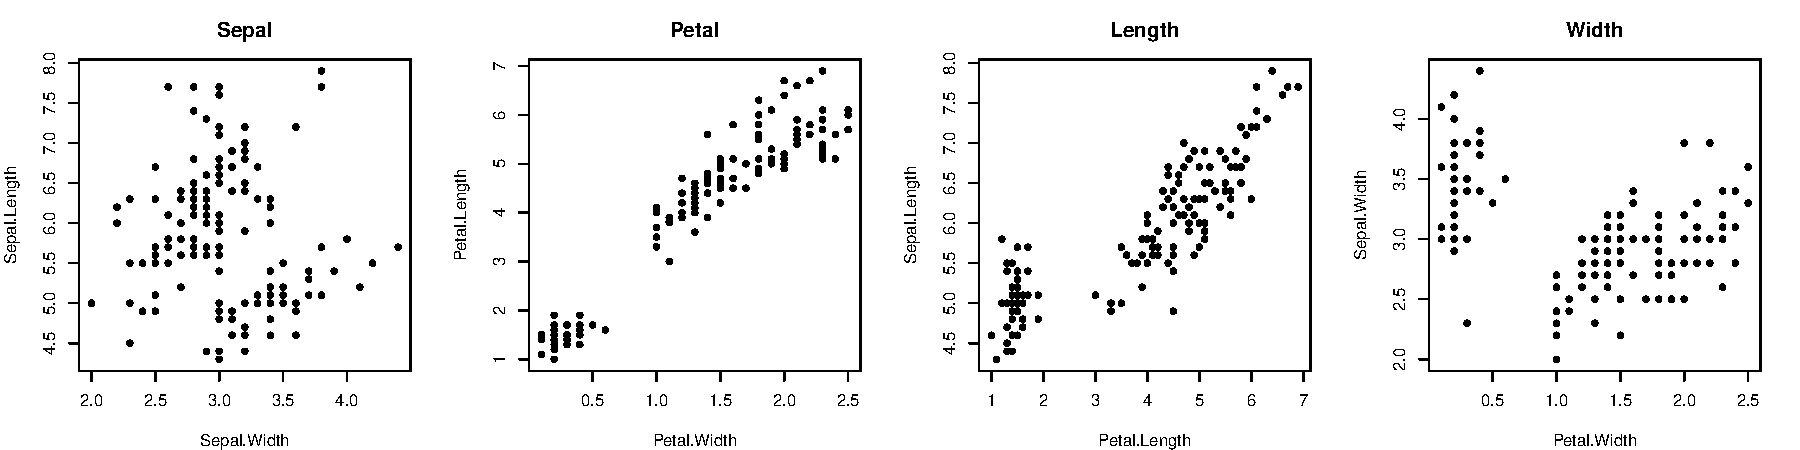
\includegraphics[width=11cm]{../../Graphs/Iris_raw.pdf}
\end{center} 
\end{frame}
%%%%%%%%%%%%%%%%%%%%%%%%%%%%%
\begin{frame}
\frametitle{Concept}
Observation: {\tt Petal.Length} and {\tt Petal.Width} are highly correlated: if we know one, we can predict the other one.\\
\vspace{0.3cm}
To simplify the representation, we do not need these two features: replace them by their average {\tt Petal.WL = (Petal.W+Petal.L)/2}:
\begin{center}
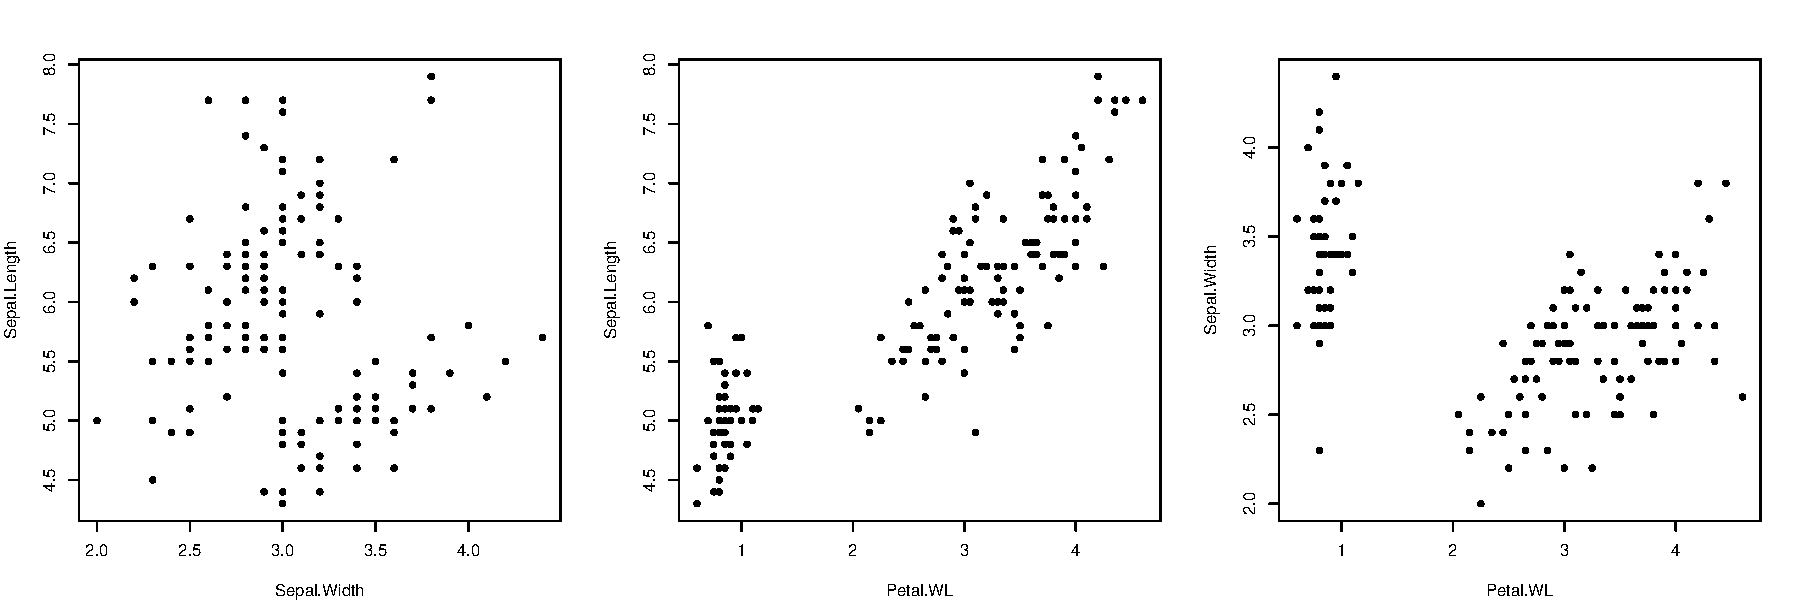
\includegraphics[width=10cm]{../../Graphs/Iris_raw2.pdf}
\end{center} 
Same observation for {\tt Petal.WL} and {\tt Sepal.Length}...
\end{frame}
%%%%%%%%%%%%%%%%%%%%%%%%%%%%%
\begin{frame}
\frametitle{Concept}
In summary, two correlated features can be replaced by one combination without keeping the information. \\
\vspace{0.3cm}
The resulting representation shows as much variance as possible: theinformation is kept.\\
\vspace{0.3cm}
This is the principle of {\bf Principal Component Analysis} (PCA).
\end{frame}
%%%%%%%%%%%%%%%%%%%%%%%%%%%%%
\section{Principal Components Analysis}
%%%%%%%%%%%%%%%%%%%%%%%%%%%%%
\begin{frame}
\frametitle{PCA}
The PCA is a method that looks for dimensions that are linear combinations of the $p$ features:
$$
a_1 x_1 + a_2 x_2 + \cdots + a_p x_p.
$$
These linear combinations are called the principal components. There are $p$ principal components. 
\end{frame}
%%%%%%%%%%%%%%%%%%%%%%%%%%%%%
\begin{frame}
\frametitle{PCA: the first component}
To find the first component (i.e. coefficients $a$), one should maximize the variance along it. That is, $a$ should be the solution to 
\begin{eqnarray*}
\max_a &&Var (a_1 x_{1} + \cdots + a_p x_{p})\\
s.t.&& \sum_j a_j^2 = 1
\end{eqnarray*}
where the variance is computed on the data set.\\
\vspace{0.2cm}
The constraint on $a$ is here because $a$ is only indicating a direction and should therefore be scaled to 1. 
\end{frame}
%%%%%%%%%%%%%%%%%%%%%%%%%%%%%
\begin{frame}
\frametitle{PCA: the first component}
As an example, let's look at a toy case where we only have 2 features $x_1$ and $x_2$ showed below. We want to represent the data in one dimension, that is, along a line (dimension reduction). The dashed line shows more variability of the data and is a better principal component than the solid line.\\
\vspace{0.2cm}
\begin{center}
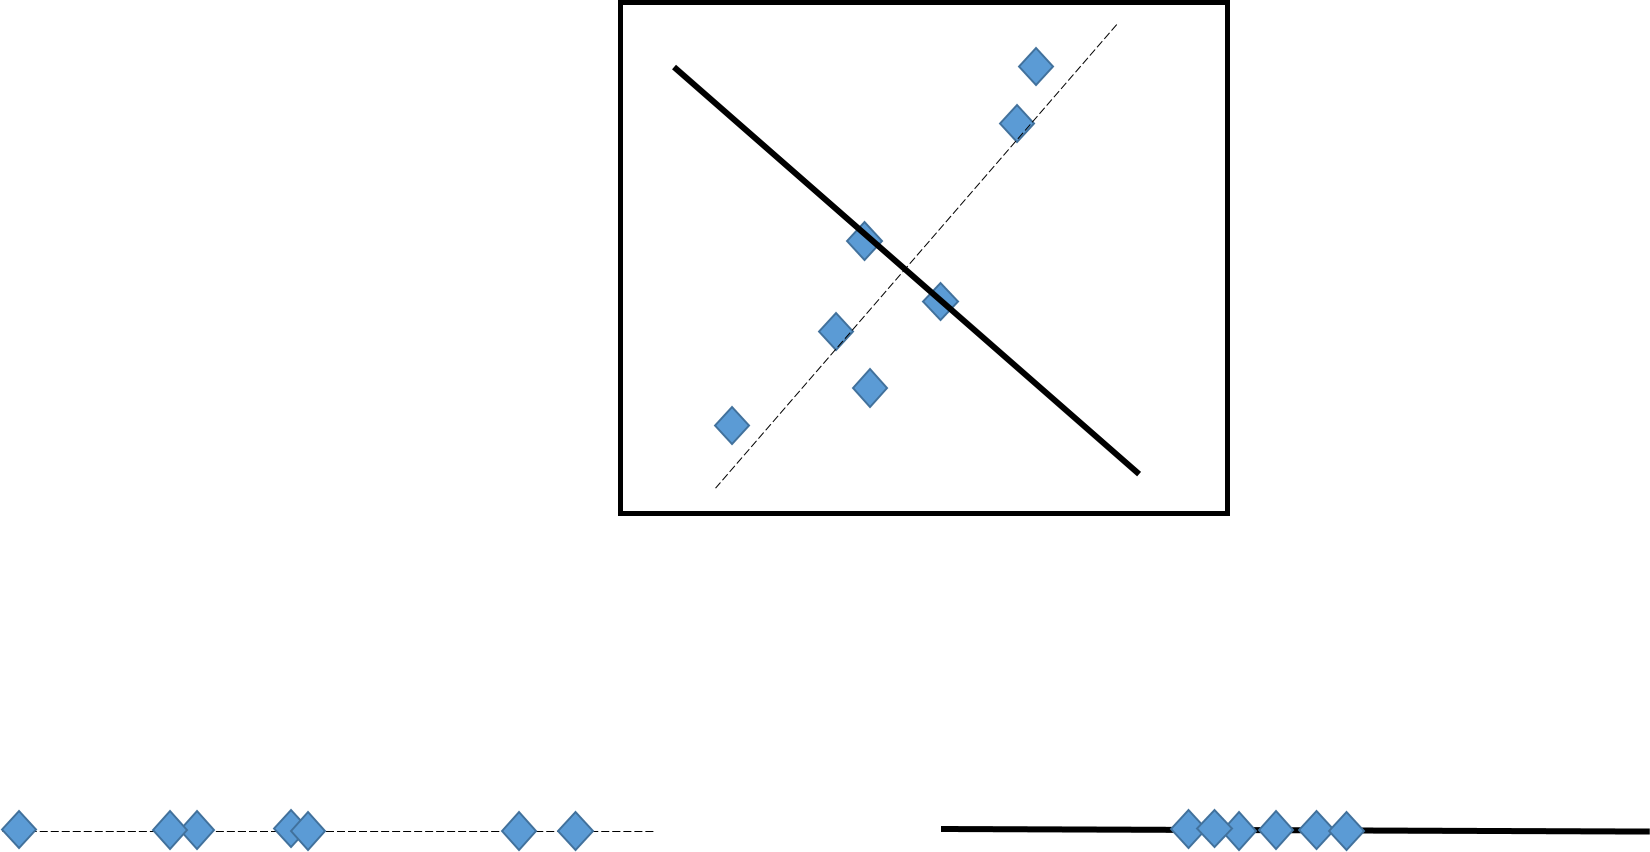
\includegraphics[width=8cm]{../../Graphs/PCA_Illustr.png}
\end{center}
\end{frame}
%%%%%%%%%%%%%%%%%%%%%%%%%%%%%
\begin{frame}
\frametitle{PCA: the first component}
When extended to $p\geq 2$ features, the principle remains the same. For a choice of $a$ with $\sum a_j^2=1$, 
\begin{itemize}
\item $z_i = a_1 x_{i1} + \cdots + a_p x_{ip}$ are computed on the data set ($i=1,\ldots,n$), \item the variance of the $z_i$ is computed.
\end{itemize}
Then this variance is maximized by changing $a$. The maximum value gives $a^{(1)}$, the first principle component.
\end{frame}
%%%%%%%%%%%%%%%%%%%%%%%%%%%%%
\begin{frame}
\frametitle{PCA: the second component, and third, etc.}
The second component $a^{(2)}$ is obtained with the same principle and the extra constraint to be orthogonal to the first one:
$$
\sum_{j=1}^p a^{(1)}_j a^{(2)}_j = 0.
$$
The procedure is repeated until $p$ principal components are found (each one is orthogonal to all the previous ones). \\
\vspace{0.3cm}
Note: the result can be quickly obtained by computing the {\bf spectral decomposition} of the variance matrix of the data. 
\end{frame}
%%%%%%%%%%%%%%%%%%%%%%%%%%%%%
\begin{frame}
\frametitle{PCA: scaling}
Before computing the PCA, the data can be standardized. Like any standardization, this is a choice of the user, which depends strongly on the application and on the scale (units) of the data. \\
\vspace{0.3cm}
When the data are first standardized, the spectral decomposition is made on the correlation matrix of the data. 
\end{frame}
%%%%%%%%%%%%%%%%%%%%%%%%%%%%%
\begin{frame}
\frametitle{PCA: projection}
For each PC $j$, we have the corresponding projections of the data $x_i$
$$
z_i^{(j)} = a^{(j)}_1 x_{i1} + \cdots + a^{(j)}_p x_{ip}.
$$
We thus have a new data set $z$ whose column are the projection of the features $x$ on the PCA's. These new features $z_1, \ldots, z_p$ can be used 
\begin{itemize}
\item for data representation (dimension reduction),
\item to describe the dependence between the features (factor analysis).  
\end{itemize}
\end{frame}
%%%%%%%%%%%%%%%%%%%%%%%%%%%%%
\begin{frame}
\frametitle{PCA: variance proportion}
By construction, the first principal component $z_1$ has larger variance than $z_2$ and so on. Also, by construction, the total of the variance is preserved:
$$
\sum_{j=1}^p var(x_j) = \sum_{j=1}^p var(z_j).
$$
The proportion of the total variance explained by the PC $z_j$ is thus
$$
var(z_j)/\sum_{j'=1}^p var(z_{j'}).
$$
It represents how well the data are represented on the component $z_j$.
\end{frame}
%%%%%%%%%%%%%%%%%%%%%%%%%%%%%
\begin{frame}
\frametitle{PCA: example}
\begin{center}
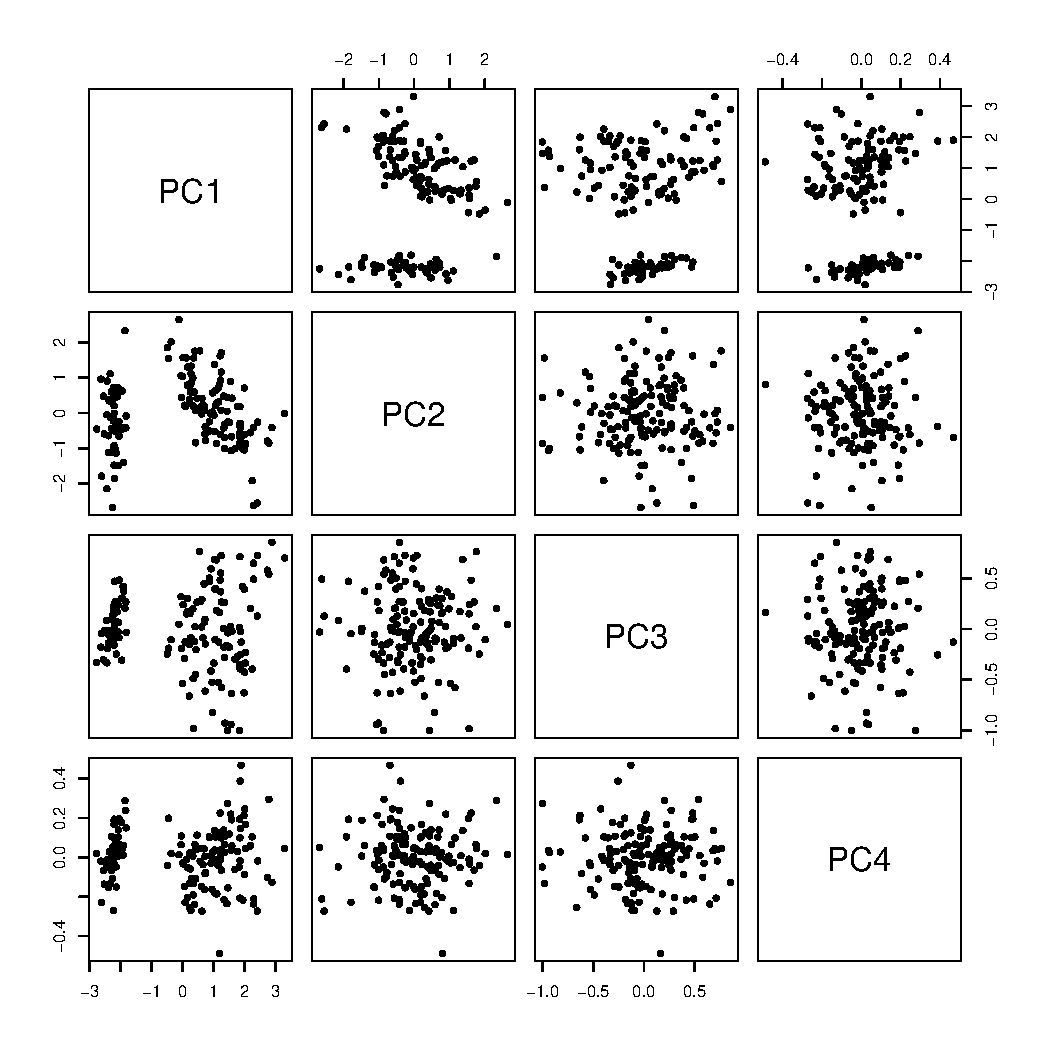
\includegraphics[width=7cm]{../../Graphs/Iris_pca.pdf}
\end{center}
\end{frame}
%%%%%%%%%%%%%%%%%%%%%%%%%%%%%
\begin{frame}[fragile]
\frametitle{PCA: example}
\scriptsize
\begin{verbatim}
> iris.pca <- PCA(iris[,-5], graph=FALSE) 
> summary(iris.pca)

Call:
PCA(X = iris[, -5], graph = FALSE) 


Eigenvalues
                       Dim.1   Dim.2   Dim.3   Dim.4
Variance               2.918   0.914   0.147   0.021
% of var.             72.962  22.851   3.669   0.518
Cumulative % of var.  72.962  95.813  99.482 100.000
\end{verbatim}
\normalsize
Together, PC1 and PC2 explain $95.8\%$ of the variation of the data. The scatter plot matrix shows that it is a good representation of the data with only two dimensions (PC$_1$, PC$_2$).
\end{frame}
%%%%%%%%%%%%%%%%%%%%%%%%%%%%%
\begin{frame}
\frametitle{PCA: the circle of correlations}
Correlation between the PC and the features $x$ can be computed to see how is PC is correlated to each features.
\begin{center}
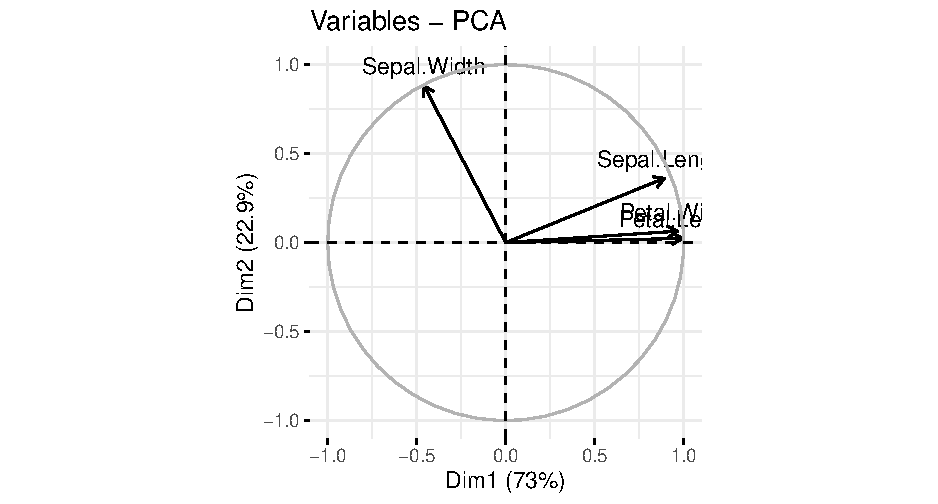
\includegraphics[width=10cm]{../../Graphs/Iris_pcacircle.pdf}
\end{center}
\end{frame}
%%%%%%%%%%%%%%%%%%%%%%%%%%%%%
\begin{frame}
\frametitle{PCA: the circle of correlations}
We see that
\begin{itemize}
\item PC$_1$ is positively and strongly correlated with petal length, petal width, and sepal length. This component summarizes these 3 features: the larger PC$_1$, the larger these 3 features.
\item PC$_2$ is (negatively) correlated with sepal width. The larger PC$_2$ the smaller this feature.
\item PC$_1$ explains $73\%$ of the total data variation. PC$_2$ explains $23\%$ of it.
\end{itemize}
With one graph, we know 
\begin{itemize}
\item which features are correlated/independent
\item how to summarize the data into two dimensions. 
\end{itemize}
\end{frame}
%%%%%%%%%%%%%%%%%%%%%%%%%%%%%
\begin{frame}
\frametitle{PCA: the $cos^2$}
The circle of correlations relates the dimensions and the features. Another view is the {\bf $cos^2$} graph. It is interpreted as the quality of the representation of the feature by the dimension. Of course this is intimately related to the correlations.
\begin{center}
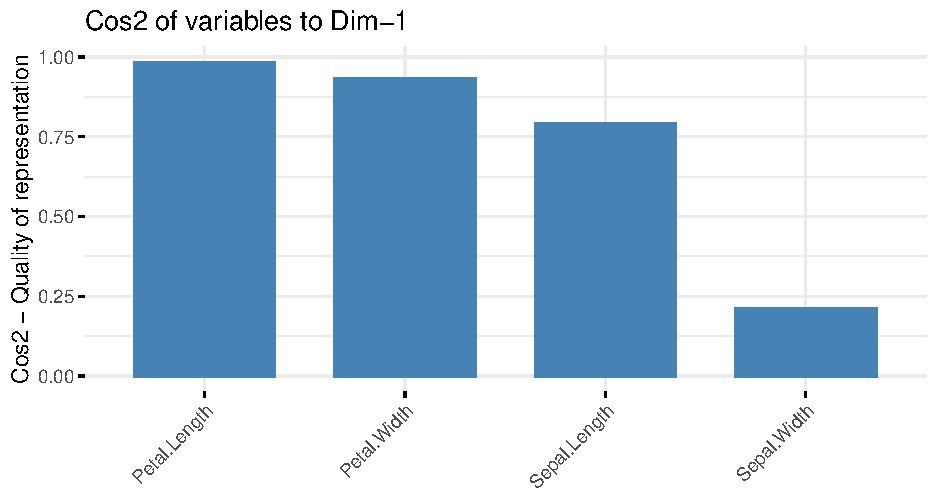
\includegraphics[width=8cm]{../../Graphs/Iris_cos2.pdf}
\end{center}
\end{frame}
%%%%%%%%%%%%%%%%%%%%%%%%%%%%%
\begin{frame}
\frametitle{PCA: the biplot}
The {\bf biplot} shows a {\bf map of the individuals} in the dimensions and adds the circle of correlations. 
\begin{center}
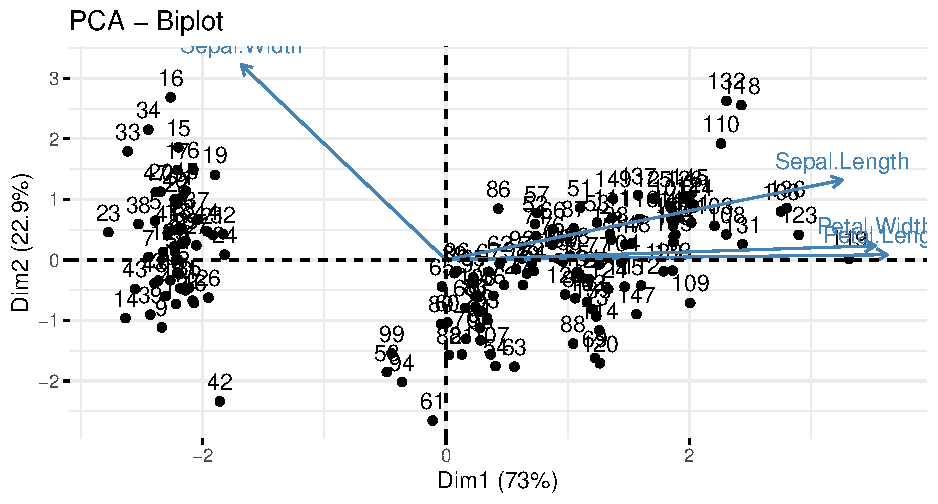
\includegraphics[width=9cm]{../../Graphs/Iris_biplot.pdf}
\end{center}
\end{frame}
%%%%%%%%%%%%%%%%%%%%%%%%%%%%%
\begin{frame}
\frametitle{PCA: the biplot}
For example, we can conclude that
\begin{itemize}
\item instance 61 has a sepal width smaller than the average (large PC$_2$) and an average PC$_1$ (which indicates an average petal length, width and sepal length).
\item instance 119 has an average sepal width but a large PC$_1$, i.e. petal length and width and sepal length.
\item Two clusters can be observed and are well separated by PC$_1$ (in fact these clusters correspond to species here).
\end{itemize}
\end{frame}
%%%%%%%%%%%%%%%%%%%%%%%%%%%%%
\begin{frame}
\frametitle{PCA: number of components}
Here, two components explain more than $95\%$ of the data variability. Sometimes, more components are needed.\\ 
\vspace{0.2cm}
One way to set the number of components is to target the proportion of explained variance: often between $75\%$ and $95\%$. \\
\vspace{0.2cm}
If the features are independent, this number is likely to be large. If the features are correlated, this number will be smaller.\\
\vspace{0.2cm}
The {\bf screeplot} may help.
\end{frame}
%%%%%%%%%%%%%%%%%%%%%%%%%%%%%
\begin{frame}
\frametitle{PCA: the screeplot}
\begin{center}
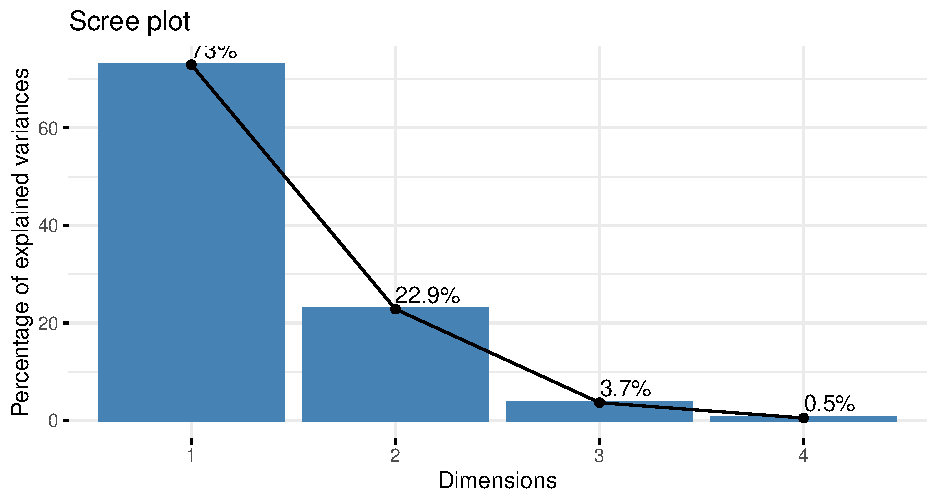
\includegraphics[width=9cm]{../../Graphs/Iris_scree.pdf}
\end{center}
\end{frame}
%%%%%%%%%%%%%%%%%%%%%%%%%%%%%
\begin{frame}
\frametitle{PCA and machine learning}
In the context of machine learning, PCA is often used 
\begin{itemize}
\item To inspect the data, find/explain clusters, find dependence between the features. {\bf PCA} can be used for {\bf EDA}.
\item To diminish the number of features when there are too many: dimension reduction $=>$ only keep few first PC.
\end{itemize}
\end{frame}
%%%%%%%%%%%%%%%%%%%%%%%%%%%%%
\begin{frame}
\frametitle{Categorical data}
PCA can only be performed on {\bf numerical features}. When categorical features are also included in the analysis,
\begin{itemize}
\item for ordinal data, quick and dirty solution: modalities can be mapped to numbers ($1,2,\ldots$) respecting their order,
\item for nominal data: there is no correct solution; especially replacing by numbers is {\bf incorrect}.
\end{itemize}
With only categorical data, {\bf (Multiple) Correspondence Analysis} is a solution. And for mixed data type (categorical and numerical), {\bf Factor Analysis of Mixed Data} (FAMD) is a solution. However, they are not adapted to large data set.
\end{frame}
%%%%%%%%%%%%%%%%%%%%%%%%%%%%%
\section{Auto-encoders}
%%%%%%%%%%%%%%%%%%%%%%%%%%%%%
\begin{frame}
\frametitle{Principle}
PCA is a "linear" technique, based on the explanation of the correlation between the features. Auto-encoder are neural network. The idea is to train a model that recovers an instance with an intermediate layer of lower dimension than the number of features.\\
\begin{center}
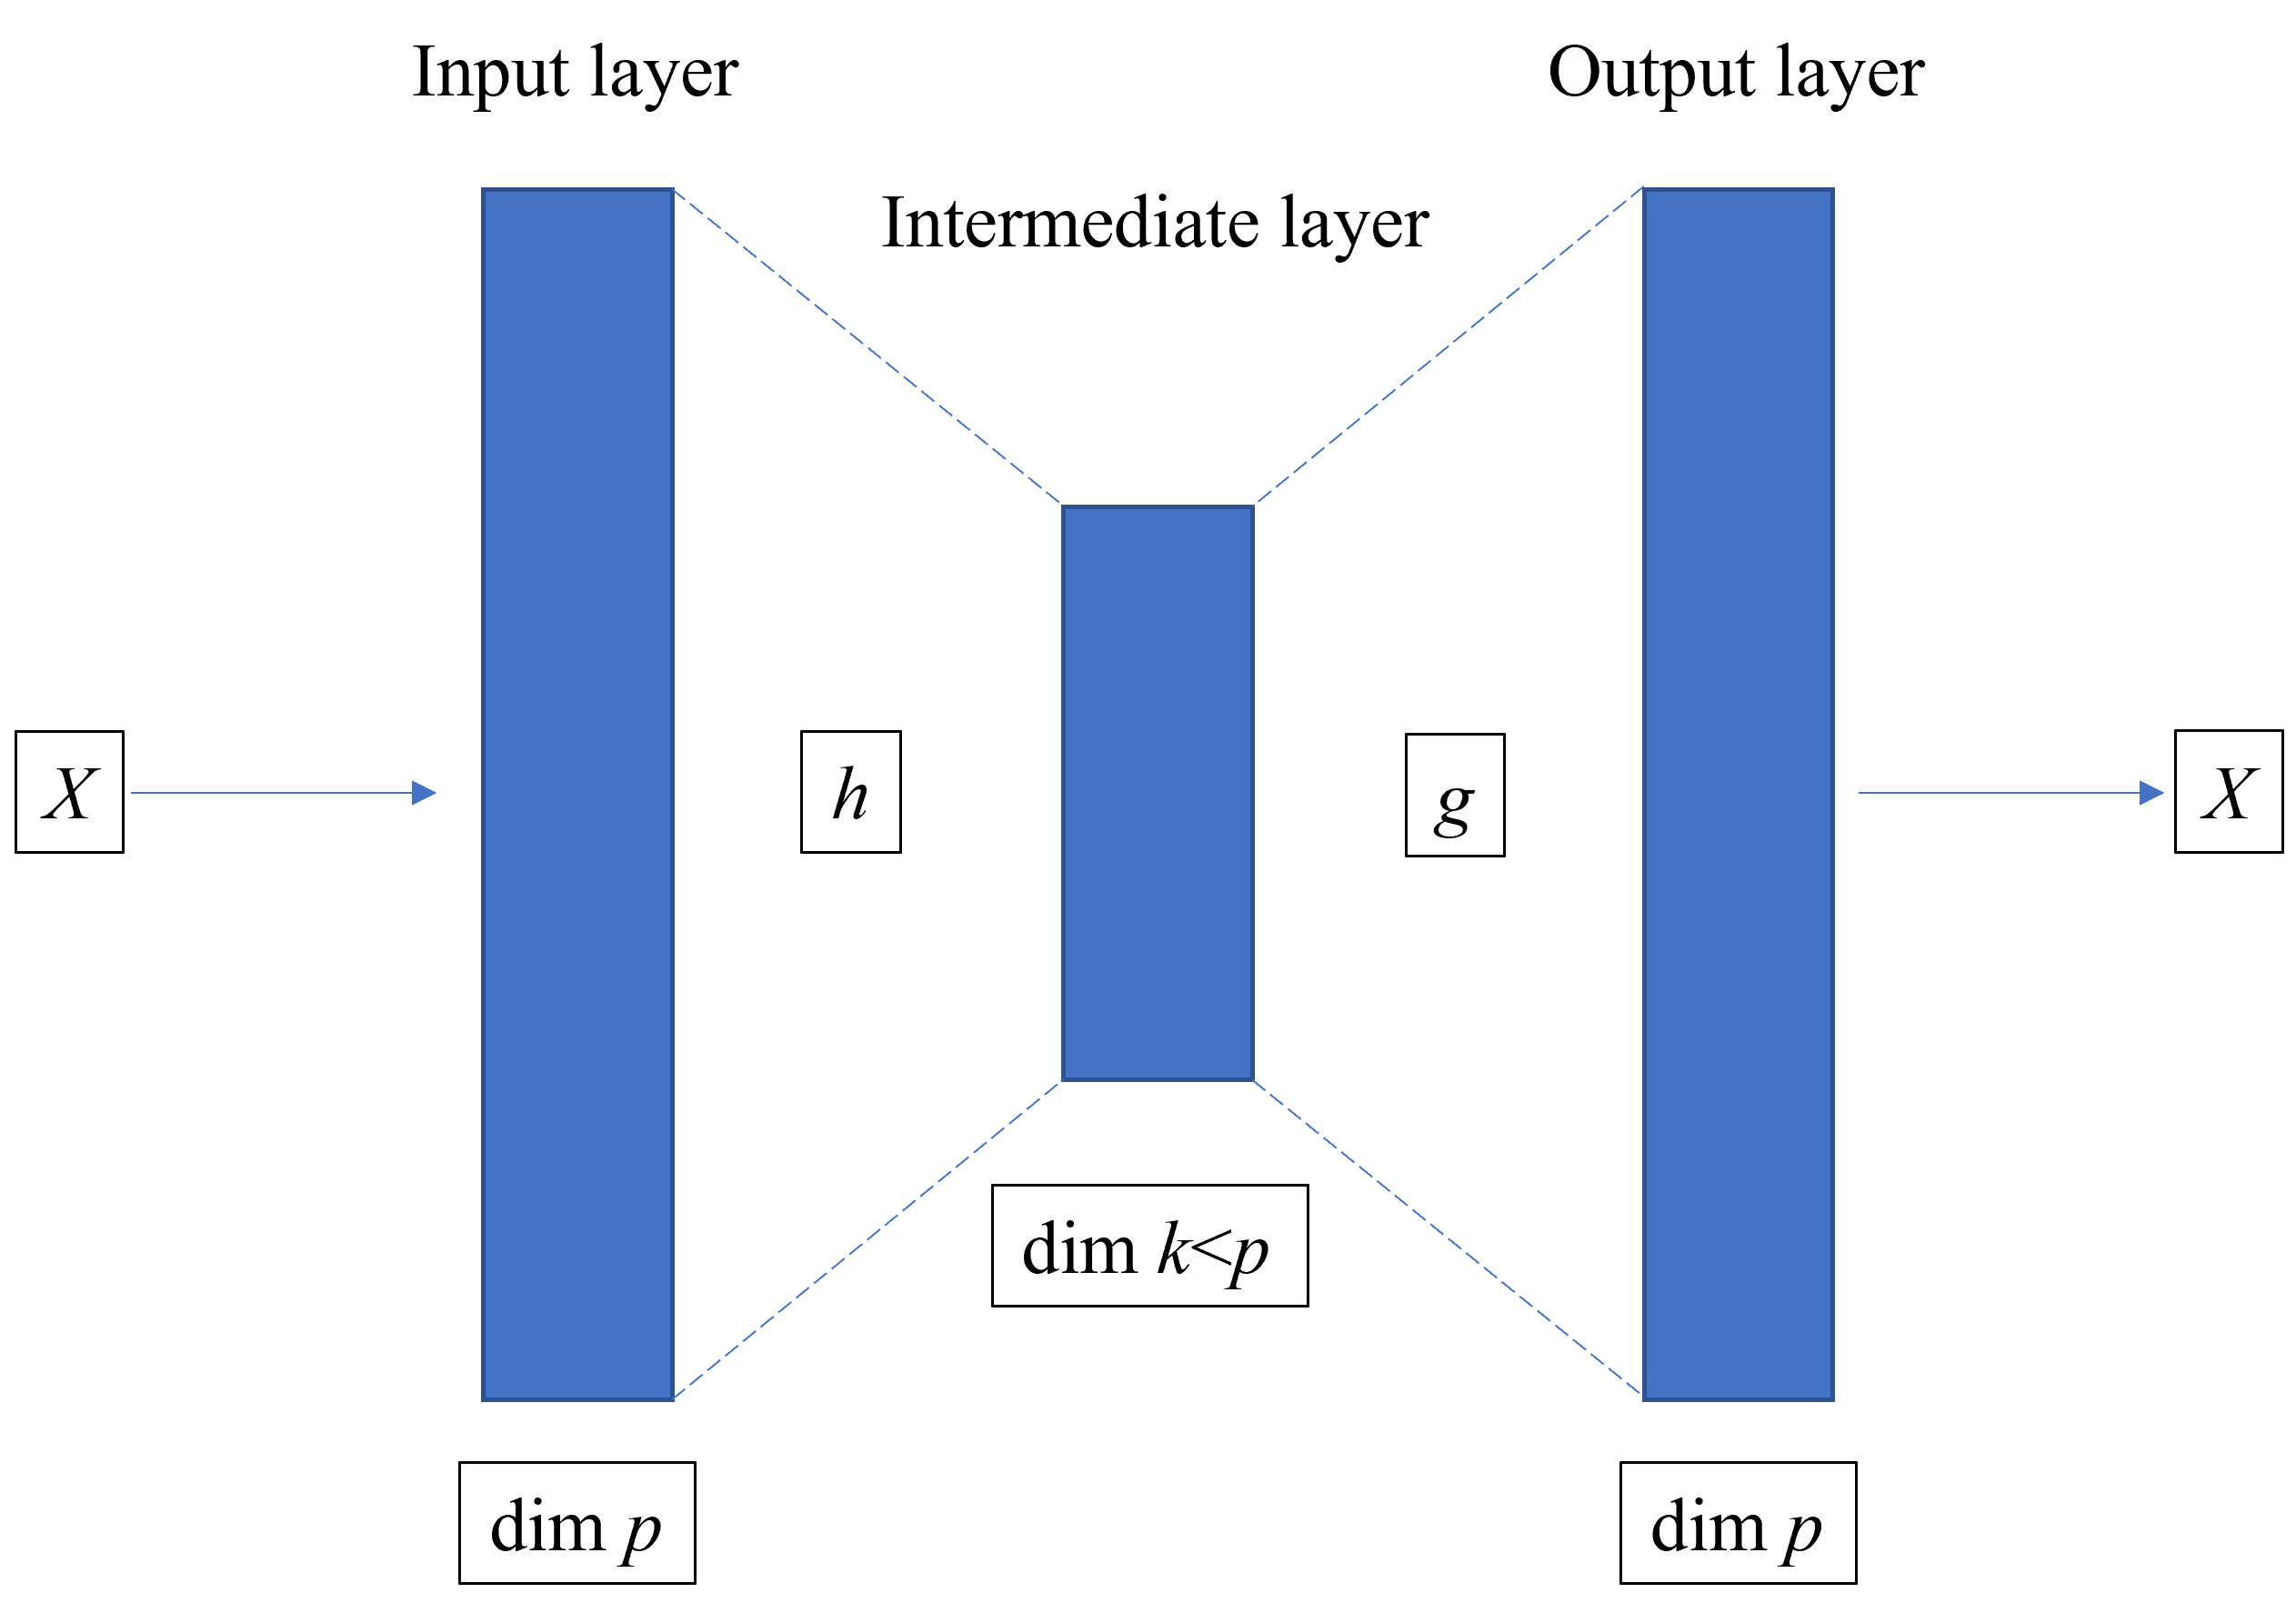
\includegraphics[width=7cm]{../../Graphs/autoencod_illustr.png}
\end{center}
\end{frame}
%%%%%%%%%%%%%%%%%%%%%%%%%%%%%
\begin{frame}
\frametitle{encoder + decoder = autoencoder}
\begin{itemize}
\item The input and the output (response) are the same instance ($X$), of dimension $p$.
\item The intermediate layer (at least one) is of dimension $k<p$.
\item The model is trained to recover $X$ ate the end.
\end{itemize}
If, after traning, the model can recover $X$ from $X$, then it can recover $X$ from its image in the intermediate layer $h(X)$. Thus, only $p$ dimensions would be needed to recover $X$. \\
\vspace{0.2cm}
Thus, 
\begin{itemize}
\item the left part of the NN {\bf encodes} $X$ in its lower-dimension version $h(X)$
\item the right part of the NN {\bf decodes} $h(X)$ in an output $g(h(X))$, hopefully close to the original image $X$.
\end{itemize}
The better this final image the better the encoding/decoding:
$$
g(h(X)) \stackrel{?}{\approx} X.
$$
\end{frame}
%%%%%%%%%%%%%%%%%%%%%%%%%%%%%
\begin{frame}
\frametitle{Autoencoder vs PCA}
In ML, often autoencoder are used to 
\begin{itemize}
\item Reduce the noise in the data (smoothing)
\item Reduce the memory needed (compressing)
\item Represent the data (dimension reduction)
\end{itemize}
Unlike PCA, autoencoder do not provide interpretation of the dimensions, which dimension is the most important, etc.\\
\vspace{0.3cm}
On the other hand, autoencoders can produce better final representation of the data: the recovery of $X$ with $k$ components is better than with PCA.
\end{frame}
%%%%%%%%%%%%%%%%%%%%%%%%%%%%%
\begin{frame}
\frametitle{Interpretability}
Like PCA make two-dimensional plots to discover pattern. Below, autoencoder (see example file) with 3-node intermediate-layer:
\begin{center}
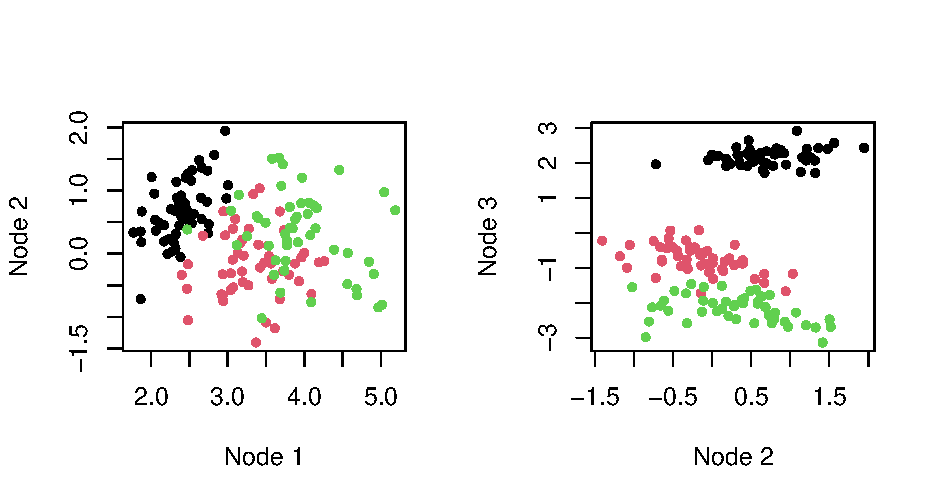
\includegraphics[width=9cm]{../../Graphs/Iris_AE_embed.pdf}
\end{center}
\end{frame}
%%%%%%%%%%%%%%%%%%%%%%%%%%%%%
\begin{frame}
\frametitle{Interpretability}
Relate each component of $h(X)$ to each component of $X$ using variable importance (or another technique). Below, Node 1 to 3 (left to right; top to bottom).
\begin{center}
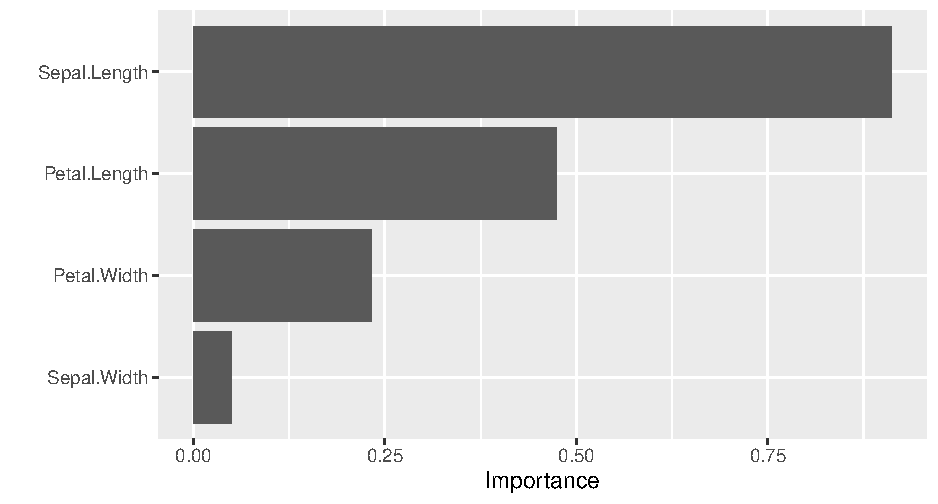
\includegraphics[width=5cm]{../../Graphs/Iris_AE_VImp1.pdf}
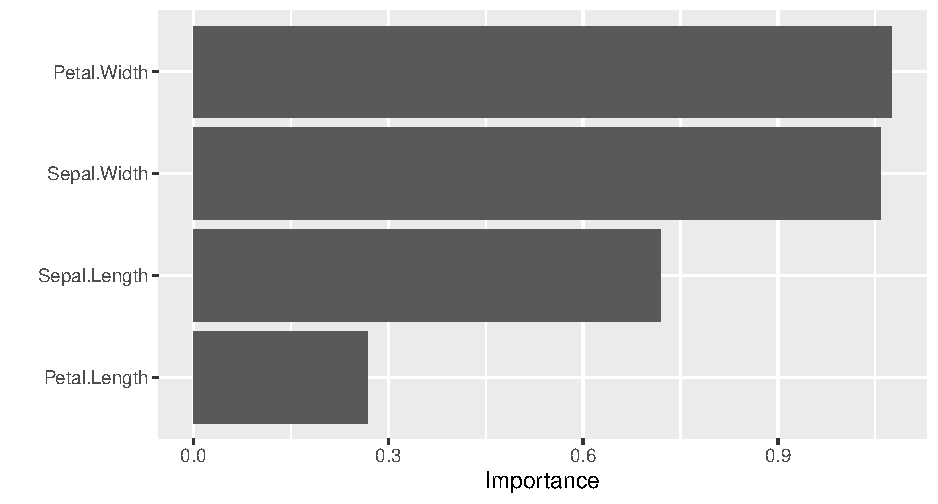
\includegraphics[width=5cm]{../../Graphs/Iris_AE_VImp2.pdf}
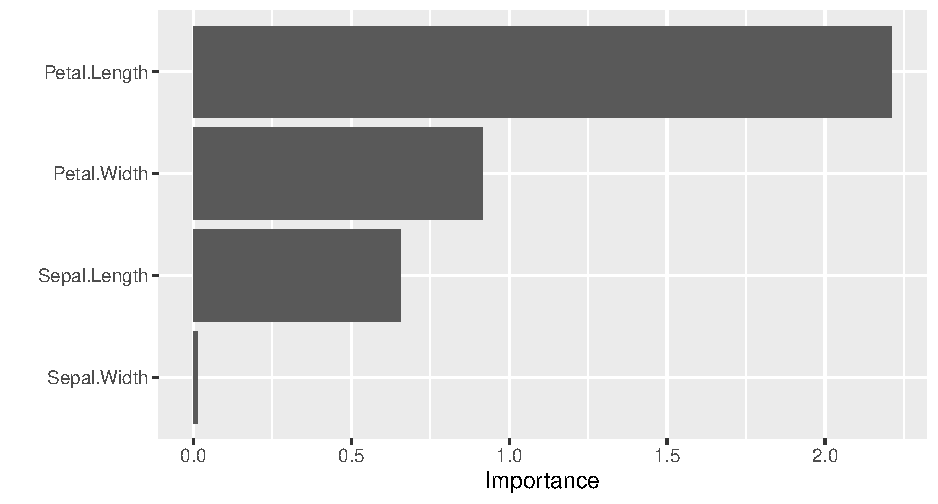
\includegraphics[width=5cm]{../../Graphs/Iris_AE_VImp3.pdf}
\end{center}
\end{frame}
%%%%%%%%%%%%%%%%%%%%%%%%%%%%%
%%%%%%%%%%%%%%%%%%%%%%%%%%%%%
\end{document}

\section{Numerical, categorical data}
%%%%%%%%%%%%%%%%%%%%%%%%%%%%%
\begin{frame}
\frametitle{Categorical features}
For categorical features, using dummy variables with PCA usually {\bf do not} provide good results.\\
\vspace{0.2cm}
For pure categorical data analysis, the technique similar to PCA is {\bf Multiple Correspondence Analysis} (MCA). 
\begin{itemize}
\item Based on spectral decomposition and interpretation of its component (mathematics are very similar to PCA)
\item Not based on the correlation matrix but a the contingency matrix (variance is replaced by inertia).
\item Different interpretations as features are related through their modalities which is more complex than just correlations.
\end{itemize}
We do not have time in this course to see MCA in details. In the following, we see how to interpret it.
\end{frame}
%%%%%%%%%%%%%%%%%%%%%%%%%%%%%
\begin{frame}
\frametitle{MCA Interpretation}
The equivalent of the correlation circle is a factor map (i.e., modality of the features).

\end{frame}

\section{Factor Analysis of Mixed Data}
%%%%%%%%%%%%%%%%%%%%%%%%%%%%%
\begin{frame}
\frametitle{Concept}
Much less known than PCA, FAMD is a mixture of two techniques
\begin{itemize}
\item PCA for numerical features,
\item {\bf Multiple Correspondence Analysis} (MCA) for categorical features.
\end{itemize}
For sake of time, we do not see MCA in detail in this course. The focus is made on the interpretation and its use for dimensional reduction. \\
\vspace{0.3cm}
One must pay attention to the subtleties of different interpretations between the part of numerical features (PCA) and the one for categorical features (MCA). 
\end{frame}
%%%%%%%%%%%%%%%%%%%%%%%%%%%%%
\begin{frame}[fragile]
\frametitle{Only categorical data}
To illustrate, we create an artificial {\tt iris} data containing
\begin{itemize}
\item Length (S/M/L): category of length (sum of petal and sepal length),
\item Width (S/M/L): category of width (sum of petal and sepal width),
\item Species: the original feature; used as supplementary variable.
\end{itemize}
The association between length and width are shown on the tables:\\
\scriptsize
\begin{columns}
\begin{column}{0.5\linewidth}
\begin{verbatim}
          Width
Length      Width_L Width_M Width_S
  Length_L  0.8889  0.2000  0.0000
  Length_M  0.1111  0.5375  0.2558
  Length_S  0.0000  0.2625  0.7442
\end{verbatim}
\end{column}
\vrule
\hspace{0.2cm}
\begin{column}{0.5\linewidth}
\begin{verbatim}
          Width
Length     Width_L Width_M Width_S
  Length_L 0.60000 0.40000 0.00000
  Length_M 0.05263 0.75439 0.19298
  Length_S 0.00000 0.39623 0.60377
\end{verbatim}
\end{column}
\end{columns}
\normalsize
\end{frame}
%%%%%%%%%%%%%%%%%%%%%%%%%%%%%
\begin{frame}
\frametitle{Only categorical data}
MCA\footnote{With only categorical variables, FAMD is simply an MCA.} builds artificial dimension that locates width and length modalities reflecting the previous associations:
\begin{itemize}
\item Large width is associated with large length
\item Small width is associated with small length
\item Medium width and medium length (proportions) are in-between large and small width and length.
\end{itemize}
Similar to the PCA, these dimensions can be represented on a map, associated to the modalities of the variables, explains a proportion of the information of the data. Unlike PCA, the information is not measure by variance but by the {\bf inertia}.\\
\vspace{0.3cm}
Because proportions sum up to 1, there are $(3-1)\times (3-1) = 4$ possible dimensions. 
\end{frame}
%%%%%%%%%%%%%%%%%%%%%%%%%%%%%
\begin{frame}
\frametitle{Only categorical data}
The scree plot shows the percentage of inertia explained by each dimension.
\begin{center}
\includegraphics[width=7cm]{../../Graphs/FAMD_screeplot.pdf}
\end{center}
\end{frame}
%%%%%%%%%%%%%%%%%%%%%%%%%%%%%
\begin{frame}
\frametitle{Only categorical data}
\small
The plots of the contributions shows the contributions of each variable (Length and Width) to the dimensions (1 and 2).
\normalsize
\begin{columns}
\begin{column}{0.55\textwidth}
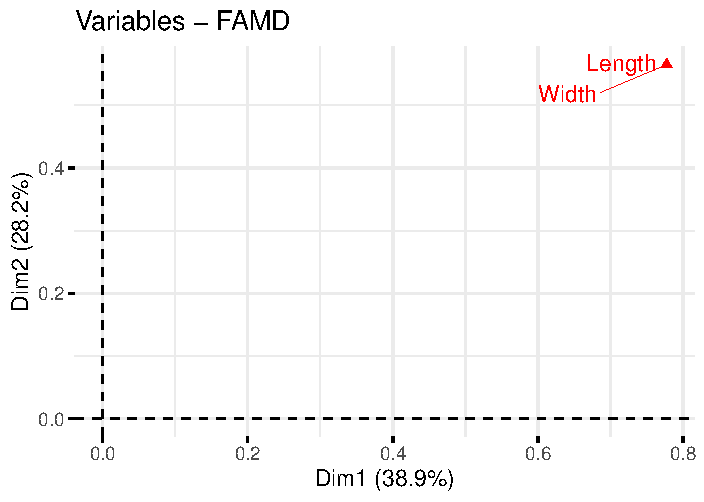
\includegraphics[width=6cm]{../../Graphs/FAMD_contrib_xy.pdf}
\end{column}
\begin{column}{0.45\textwidth}
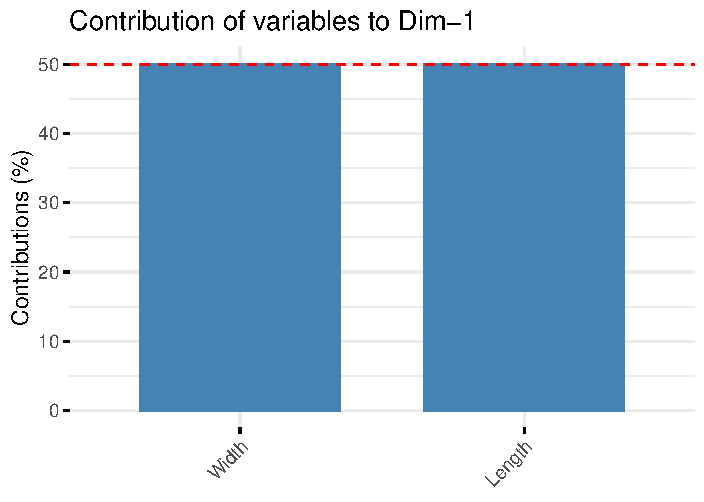
\includegraphics[width=4.5cm]{../../Graphs/FAMD_contrib_x.pdf}\\
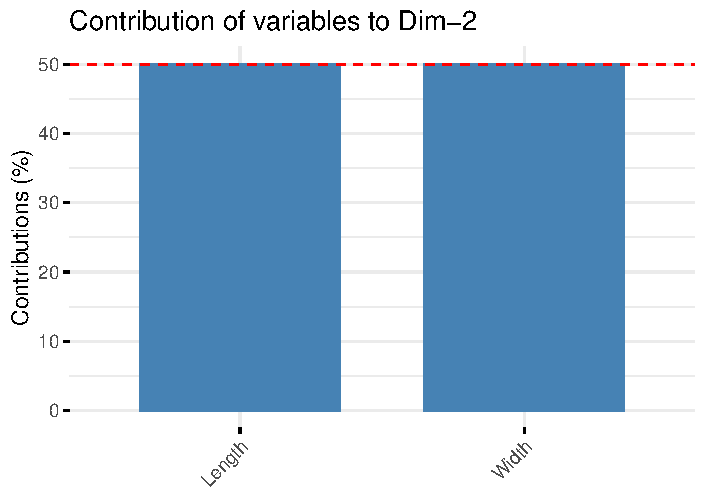
\includegraphics[width=4.5cm]{../../Graphs/FAMD_contrib_y.pdf}
\end{column}
\end{columns}
\end{frame}
%%%%%%%%%%%%%%%%%%%%%%%%%%%%%
\begin{frame}
\frametitle{Only categorical data}
The plot of the modalities locates the modalities of each variable on the map of the dimensions.
\begin{center}
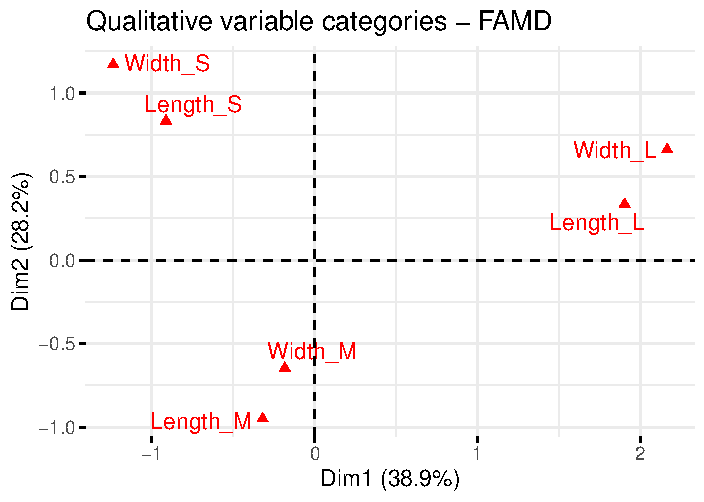
\includegraphics[width=7cm]{../../Graphs/FAMD_quali.pdf}
\end{center}
\end{frame}
%%%%%%%%%%%%%%%%%%%%%%%%%%%%%
\begin{frame}
\frametitle{Only categorical data}
The biplot of the individuals and modalities relates the observations. Below we added the species\footnote{Supplementary variables not used in the FAMD.}.
\begin{center}
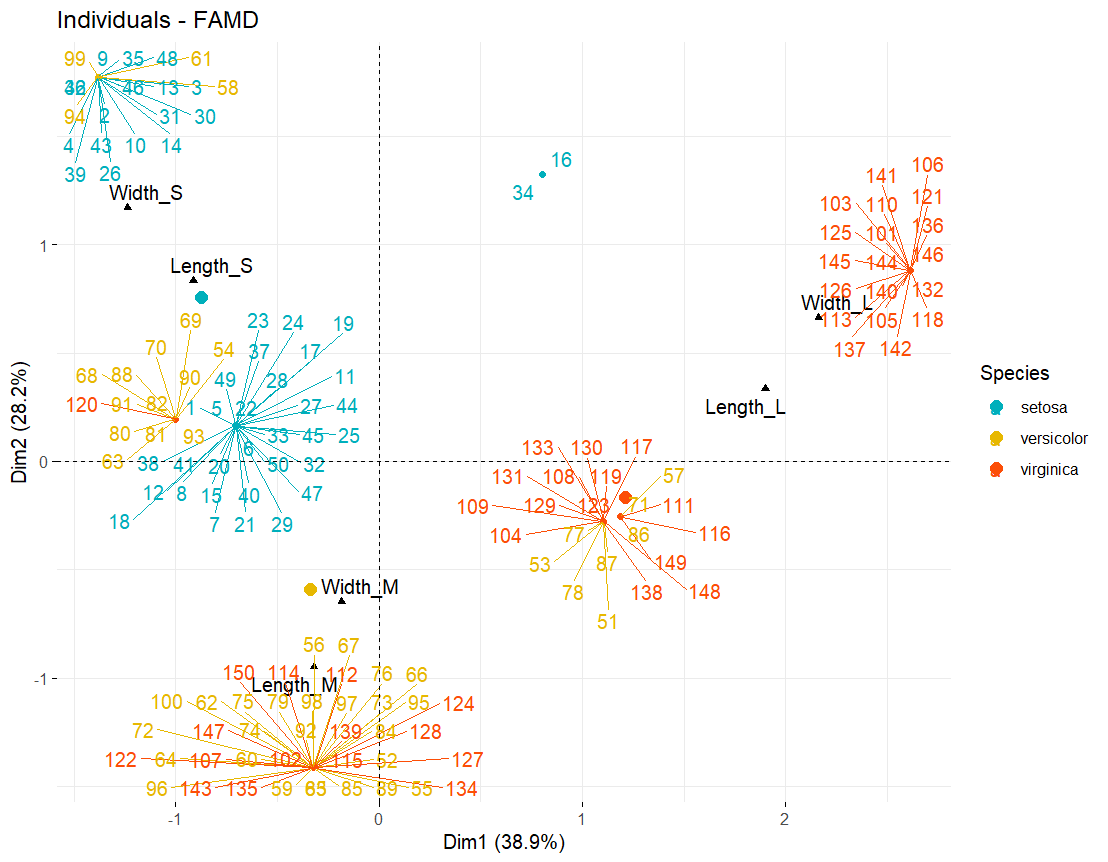
\includegraphics[width=7cm]{../../Graphs/FAMD_biplot_species.png}
\end{center}
\end{frame}
%%%%%%%%%%%%%%%%%%%%%%%%%%%%%
\begin{frame}
\frametitle{Mixed data}

\end{frame}
%%%%%%%%%%%%%%%%%%%%%%%%%%%%%
